\documentclass[11pt,letterpaper]{article}

% ---------------------------------------------------------------
% Paquetes
% ---------------------------------------------------------------
\usepackage[utf8]{inputenc}
\usepackage[T1]{fontenc}
\usepackage[spanish,es-tabla,es-nodecimaldot]{babel}
\usepackage{lmodern}
\usepackage{microtype}
\usepackage[margin=2.0cm]{geometry}
\usepackage{graphicx}
\usepackage{float}
\usepackage{booktabs}
\usepackage{tabularx}
\usepackage{longtable}
\usepackage{array}
\usepackage{multirow}
\usepackage{xcolor}
\usepackage{colortbl}
\usepackage{listings}
\usepackage{caption}
\usepackage{subcaption}
\usepackage{enumitem}
\usepackage{amsmath}
\usepackage{fancyhdr}
\usepackage{titlesec}
\usepackage{pifont}
\usepackage{tikz}
\usetikzlibrary{positioning,fit,backgrounds,arrows.meta,shapes.geometric}
\usepackage{hyperref}

\definecolor{utbblue}{HTML}{0B1F4D}
\definecolor{azure}{HTML}{0078D4}
\definecolor{codebg}{HTML}{F5F7FA}
\definecolor{okgreen}{HTML}{15803D}
\definecolor{badred}{HTML}{B91C1C}

\hypersetup{colorlinks=true,linkcolor=utbblue,urlcolor=azure,citecolor=utbblue}
\captionsetup{font=small,labelfont=bf}
\setlist{itemsep=2pt,topsep=3pt}
\renewcommand{\arraystretch}{1.18}
\setlength{\emergencystretch}{3em}
\newcolumntype{Y}{>{\raggedright\arraybackslash}X}

\titleformat{\section}{\Large\bfseries\color{utbblue}}{\thesection.}{0.5em}{}
\titleformat{\subsection}{\large\bfseries\color{utbblue}}{\thesubsection}{0.5em}{}

\lstdefinestyle{tf}{
  basicstyle=\ttfamily\footnotesize,
  backgroundcolor=\color{codebg},
  frame=single, rulecolor=\color{gray!40},
  breaklines=true, columns=fullflexible,
  keywordstyle=\color{azure}\bfseries,
  commentstyle=\color{gray}\itshape,
  stringstyle=\color{okgreen},
  morekeywords={resource,variable,output,data,locals,terraform,provider,backend,lifecycle,rule,profile},
  morecomment=[l]{\#},
  morestring=[b]",
  showstringspaces=false,
  aboveskip=6pt, belowskip=6pt
}
\lstset{style=tf}

\pagestyle{fancy}
\fancyhf{}
\fancyhead[L]{\small\color{gray}Infraestructura para TI · Taller integrador}
\fancyhead[R]{\small\color{gray}CaribeShop en Azure}
\fancyfoot[C]{\small\thepage}
\renewcommand{\headrulewidth}{0.4pt}

\newcommand{\req}[1]{\textbf{\color{azure}#1}}
\newcommand{\ok}{\textcolor{okgreen}{\ding{51}}}

% ---------------------------------------------------------------
\begin{document}

\begin{titlepage}
\centering
\vspace*{1.2cm}
\includegraphics[width=0.27\textwidth]{logo_utb}\par
\vspace{1.6cm}
{\LARGE \textsc{Universidad Tecnológica de Bolívar}\par}
\vspace{1.2cm}
{\Large \textsc{Infraestructura para TI}\par}
\vspace{0.5cm}
{\Large NRC: 1216\par}
\vspace{1.4cm}
{\Large \bfseries TALLER INTEGRADOR: Plataforma Segura, Escalable y\\[0.3em]
Altamente Disponible en Azure — Caso CaribeShop\par}
\vspace{0.4cm}
{\large Informe final\par}
\vspace{1.2cm}
{\large\itshape
Santiago Payares González\\[0.3em]
Cristian Matteo Benitez Montes\\[0.3em]}
\vspace{1.4cm}
{\large Revisado por\\[0.3em] Prof. Rafael Enrique Monterroza Barrios\par}
\vfill
{\large Noviembre de 2026\par}
\end{titlepage}

\newcommand{\RES}[1]{\textbf{\color{badred}[#1]}}
% =================================================================
\section{Introducción y alcance}
% =================================================================
CaribeShop es una tienda en línea de Cartagena que el año pasado tuvo tres problemas: se cayó
durante una promoción porque no aguantó la demanda, volvió a caerse porque dependía de una sola
máquina virtual, y una auditoría encontró la contraseña de la base de datos dentro del código y
el acceso remoto (SSH) abierto a Internet.

Este informe describe cómo diseñamos, desplegamos y probamos en Microsoft Azure una plataforma
que corrige esos tres problemas: es \textbf{segura}, \textbf{crece sola} cuando aumenta la demanda
y \textbf{sigue funcionando} cuando falla una de sus partes. Toda la infraestructura se creó con
código (Terraform) y cada requisito se comprobó con una prueba.

\begin{itemize}
  \item \textbf{Repositorio:} \url{https://github.com/AgEnt3P18/caribeshop-taller-integrador}
  \item \textbf{Herramientas:} Terraform, Azure CLI, GitHub Actions, Checkov (revisión de seguridad
        del código) y Locust (pruebas de carga).
  \item \textbf{Región:} East US, repartiendo los servidores en sus tres zonas de disponibilidad.
\end{itemize}

% =================================================================
\section{Arquitectura y decisiones de diseño}
% =================================================================
La Figura~\ref{fig:arq} resume el recorrido de una visita: entra por un balanceador de carga, que
la envía a uno de los servidores sanos; los servidores viven en una red privada, repartidos en
tres zonas, y consultan la contraseña en un Key Vault. Todo queda registrado para monitoreo.

\begin{figure}[H]
\centering
\begin{tikzpicture}[
  font=\small,
  caja/.style={draw=thead, line width=0.9pt, fill=white, rounded corners=4pt, minimum height=13mm,
               minimum width=31mm, align=center},
  serv/.style={fill=turq, text=white, rounded corners=3pt, minimum width=30mm, minimum height=9mm,
               font=\small\bfseries},
  flecha/.style={-{Stealth[length=2.6mm]}, line width=1.1pt, color=thead!80}
]
\node[caja] (u) {\textbf{Clientes}\\ desde Internet};
\node[caja, right=11mm of u] (lb) {\textbf{Balanceador}\\ \textbf{de carga}\\ \footnotesize revisa cada servidor\\ \footnotesize cada 5 segundos};
\node[serv, right=17mm of lb, yshift=12mm] (v1) {Servidor · zona 1};
\node[serv, below=3mm of v1] (v2) {Servidor · zona 2};
\node[serv, below=3mm of v2] (v3) {Servidor · zona 3};
\begin{scope}[on background layer]
  \node[draw=badred!70, dashed, line width=0.9pt, rounded corners=6pt, fill=badred!4,
        fit=(v1)(v3), inner xsep=5mm, inner ysep=4mm] (red) {};
\end{scope}
\node[font=\footnotesize\bfseries, color=badred!85, anchor=south] at ([yshift=0.5mm]red.north) {Red privada · solo entra tráfico web};
\node[font=\footnotesize\itshape, color=thead, anchor=north] at ([yshift=-1mm]red.south)
  {de 2 a 4 servidores, se agregan solos};
\node[caja, right=13mm of red.east, yshift=12mm] (kv) {\textbf{Key Vault}\\ \footnotesize guarda la contraseña};
\node[caja, right=13mm of red.east, yshift=-12mm] (mon) {\textbf{Monitoreo}\\ \footnotesize registros y alertas\\ \footnotesize por correo};
\draw[flecha] (u) -- (lb);
\draw[flecha] (lb) -- (red.west |- lb);
\draw[flecha] (red.east |- kv) -- (kv);
\draw[flecha] (red.east |- mon) -- (mon);
\node[fill=thead, text=white, rounded corners=4pt, inner xsep=4mm, inner ysep=2.2mm,
      font=\footnotesize, align=center, anchor=north] (gob)
  at ([yshift=-10mm]$(u.west |- red.south)!0.5!(kv.east |- red.south)$)
  {Todo se crea con \textbf{Terraform} \quad·\quad cada cambio lo revisa \textbf{GitHub Actions + Checkov}\\
   \textbf{Azure Policy} bloquea lo prohibido \quad·\quad el estado de Terraform vive protegido en Azure};
\end{tikzpicture}
\caption{Arquitectura desplegada en Azure.}
\label{fig:arq}
\end{figure}

\begin{table}[H]
\centering\small\tablaestilo
\caption{Principales decisiones de diseño.}
\label{tab:decisiones}
\begin{tabularx}{\textwidth}{|>{\raggedright\arraybackslash\bfseries}p{4.6cm}|Y|}
\hline
\encab \hd{Qué elegimos} & \hd{Por qué} \\ \hline
Servidores en las 3 zonas de East US & Si una zona falla, las otras siguen atendiendo. Elegimos el tamaño D2s\_v4 porque era el que tenía cupo disponible en las tres zonas. \\ \hline
Balanceador de carga Standard & Revisa la salud de cada servidor y deja de enviarle tráfico si falla. Para producción se recomienda además un firewall de aplicaciones web (WAF). \\ \hline
Aplicación sin librerías externas & Así los servidores no necesitan salir a Internet, y pudimos \textbf{bloquear toda la salida}. Usa un proceso por núcleo para aprovechar toda la CPU. \\ \hline
Contraseña en Key Vault & La aplicación la lee con su propia identidad y \textbf{solo tiene permiso sobre ese único secreto}. \\ \hline
Bloqueo de salida con la red (NSG) & Solo se permite hablar con Key Vault, Monitor y Storage. Es gratis, frente a $\approx$\,USD 900/mes de un firewall dedicado. \\ \hline
Reparación automática & Si un servidor queda enfermo más de 10 minutos, Azure lo reemplaza solo. \\ \hline
Dos políticas de Azure (Deny) & Prohíben servidores con IP pública y recursos fuera de East US, sin importar desde dónde se creen. \\ \hline
\end{tabularx}
\end{table}

% =================================================================
\section{Implementación paso a paso}
% =================================================================
\begin{enumerate}
  \item \textbf{Acceso a Azure.} Iniciamos sesión con la CLI. El método por código de dispositivo
        estaba bloqueado por la seguridad predeterminada de la cuenta, así que usamos el inicio
        de sesión por navegador.
  \item \textbf{Región y tamaño.} Revisamos las cuotas de la suscripción (10 núcleos por región)
        y qué tamaños estaban disponibles en las tres zonas.
  \item \textbf{Estado de Terraform.} Creamos primero una cuenta de almacenamiento protegida, sin
        llaves de acceso, para guardar el estado de Terraform fuera de Git.
  \item \textbf{Despliegue.} Con \texttt{terraform plan} y \texttt{apply} se crearon los 33 recursos
        de una sola vez.
  \item \textbf{Configuración automática.} Cada servidor se instala solo al arrancar
        (\emph{cloud-init}); cuando cambiamos la aplicación bastó con volver a aplicar y reiniciar
        las instancias, sin entrar a ninguna máquina.
  \item \textbf{Pruebas y evidencias.} Ejecutamos las pruebas P1, P2 y P3 y guardamos los resultados
        en la carpeta \texttt{evidencias/} del repositorio.
\end{enumerate}

\textbf{Por qué el autoscale usa umbrales distintos para subir y bajar.} Agrega un servidor cuando
la CPU pasa del 70\,\% durante 5 minutos y quita uno cuando baja del 30\,\% durante 10 minutos.
Entre ambos valores no hace nada, lo que evita que agregue y quite servidores sin parar. Bajar es
más lento a propósito: quitar capacidad antes de tiempo es peor que mantenerla unos minutos más.
Tras cada acción espera 5 minutos (al subir) o 10 (al bajar), el tiempo que tarda una instancia
nueva en arrancar y estabilizarse.

% =================================================================
\section{Trazabilidad de requisitos}
% =================================================================
\begin{table}[H]
\centering\footnotesize\tablaestilo
\caption{Cada requisito, dónde se implementa y cómo se comprobó.}
\label{tab:traz}
\begin{tabularx}{\textwidth}{|>{\raggedright\arraybackslash}p{4.2cm}|>{\raggedright\arraybackslash}p{3.7cm}|Y|}
\hline
\encab \hd{Requisito} & \hd{Dónde se implementa} & \hd{Evidencia} \\ \hline
\grupo{3}{Seguridad} \\ \hline
S1 · Todo en Terraform & \texttt{providers.tf}, \texttt{bootstrap/} & Estado remoto; Git sin estado ni credenciales \\ \hline
S2 · Red mínima & \texttt{network.tf} (NSG) & Servidores sin IP pública; SSH inalcanzable \\ \hline
S3 · Key Vault & \texttt{keyvault.tf} & \texttt{/secret} muestra solo longitud y huella \\ \hline
S4 · Mínimo privilegio & \texttt{keyvault.tf} & Un único rol, limitado al secreto \\ \hline
S5 · Azure Policy & \texttt{policy.tf} & Rechazo \texttt{RequestDisallowedByPolicy} (Lst.~\ref{lst:policy}) \\ \hline
S6 · Auditoría & \texttt{monitoring.tf} & Consulta KQL de lecturas (Lst.~\ref{lst:kql}) \\ \hline
\grupo{3}{Escalamiento y alta disponibilidad} \\ \hline
E1 · Tres zonas & \texttt{compute.tf} & Instancias en zonas 1, 2 y 3 \\ \hline
E2 · Sonda de salud & \texttt{loadbalancer.tf} & Métrica de salud (Fig.~\ref{fig:p2logica}) \\ \hline
E3 · Autoscale & \texttt{compute.tf} & Historial 2\,$\rightarrow$\,4\,$\rightarrow$\,2 (Fig.~\ref{fig:stair}) \\ \hline
E4 · Reparación automática & \texttt{compute.tf} & Instancia reemplazada sola (P2.1) \\ \hline
E5 · Alertas por correo & \texttt{monitoring.tf} & Historial de alertas (Tabla~\ref{tab:alertas}) \\ \hline
\grupo{3}{DevSecOps} \\ \hline
D1 · Pipeline con Checkov & \texttt{.github/workflows/} & PR \#1 bloqueado y PR \#2 aprobado \\ \hline
D2 · Riesgos justificados & comentarios en cada recurso & Tabla~\ref{tab:riesgos} \\ \hline
D3 · Instalación automática & \texttt{cloud-init} + \texttt{app/} & Servidores listos sin pasos manuales \\ \hline
\end{tabularx}
\end{table}

% =================================================================
\section{Resultados de las pruebas}
% =================================================================
Las pruebas de carga se lanzaron con Locust desde Cartagena. Cada visita a la tienda hace
trabajar la CPU unos 40 milisegundos, para simular una página real. Los resultados completos
(CSV e informes HTML) están en la carpeta \texttt{evidencias/}.

\subsection{P1.1 ¿Cuánto aguanta un solo servidor?}
Dejamos el sistema con un único servidor y fuimos aumentando los usuarios poco a poco, de 5 en 5
y luego de 10 en 10, hasta 240.

\begin{figure}[H]
\centering
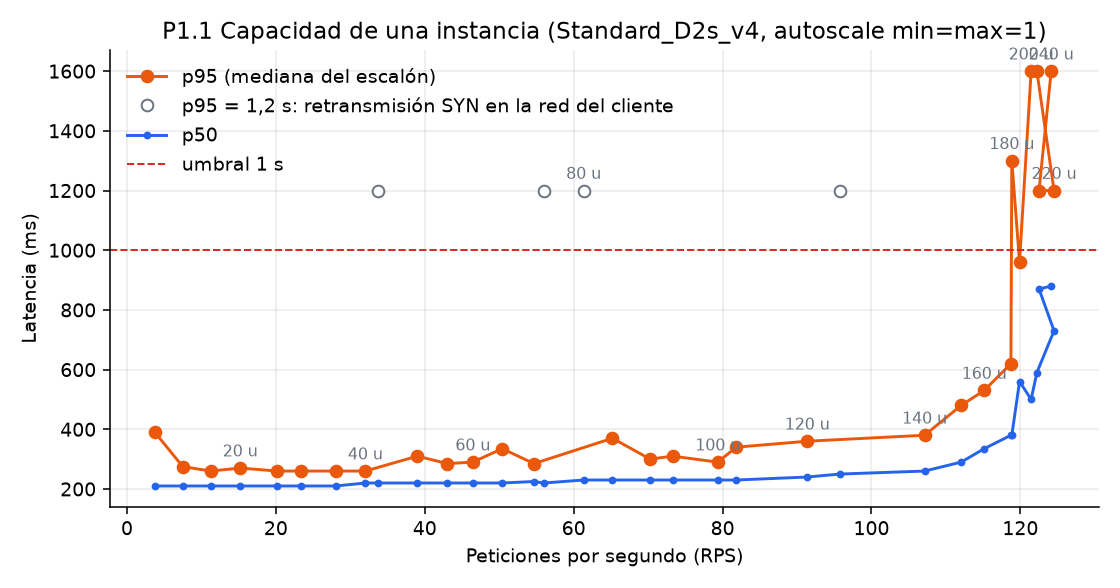
\includegraphics[width=0.82\textwidth]{figuras/p1_capacidad.png}
\caption{Tiempo de respuesta frente a peticiones por segundo con un solo servidor.}
\label{fig:cap}
\end{figure}

\begin{itemize}
  \item Un servidor atiende como máximo \textbf{unas 120 peticiones por segundo}; a partir de ahí
        la CPU llega al 98\,\% y solo crecen las esperas.
  \item \textbf{Capacidad útil: 119 peticiones/s} manteniendo el 95\,\% de las respuestas por debajo
        de 1 segundo, y \textbf{112 peticiones/s} si se exige menos de medio segundo.
  \item Al 70\,\% de CPU, el punto en que el autoscale agrega servidores, uno solo atiende unas
        60 peticiones por segundo.
  \item Los puntos grises de 1,2\,s no indican saturación: son reintentos de conexión de nuestra
        propia red doméstica. Ningún error vino del servidor.
\end{itemize}

\subsection{P1.2 ¿Escala solo cuando sube la demanda?}
Durante 35 minutos subimos la carga por escalones (de 40 a 280 usuarios) y luego la bajamos a 20,
con el autoscale configurado entre 2 y 4 servidores. En total hubo \textbf{207\,435 peticiones y
solo 0,55\,\% de errores}.

\begin{figure}[H]
\centering
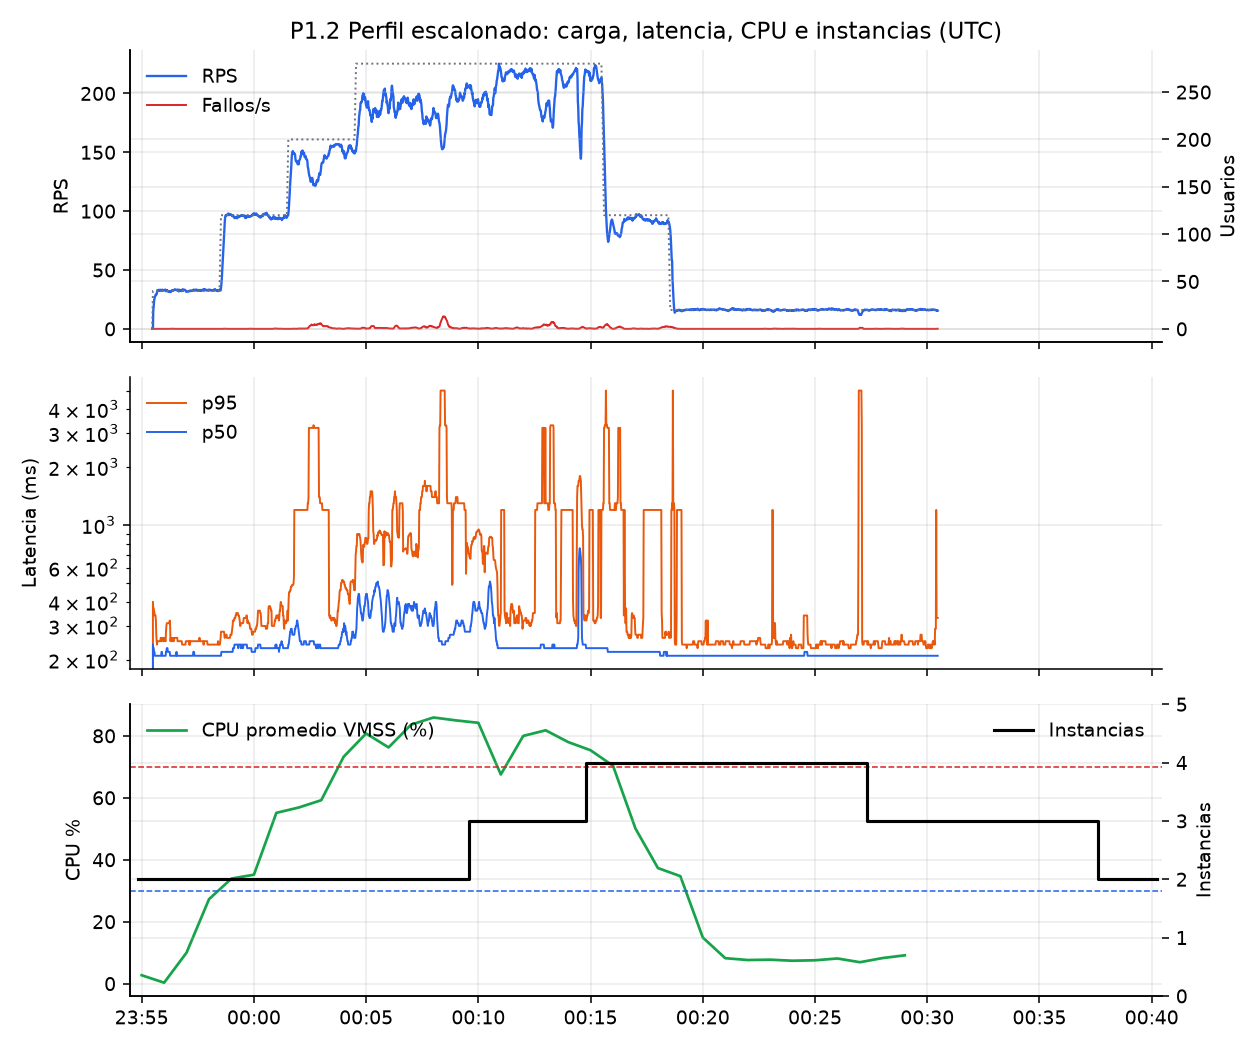
\includegraphics[width=0.86\textwidth]{figuras/p1_escalonado.png}
\caption{Carga, tiempo de respuesta, CPU y número de servidores durante la prueba (hora UTC).}
\label{fig:stair}
\end{figure}

\begin{table}[H]
\centering\small\tablaestilo
\caption{Lo que hizo el autoscale durante la prueba.}
\label{tab:autoscale}
\begin{tabular}{|c|c|p{6.4cm}|c|}
\hline
\encab \hd{Hora (UTC)} & \hd{Servidores} & \hd{Motivo} & \hd{Tardó} \\ \hline
00:09 & 2 $\rightarrow$ 3 & La CPU pasó del 70\,\% a las 00:04 & 5 min 19 s \\ \hline
00:14 & 3 $\rightarrow$ 4 & La CPU seguía alta tras la espera de 5 min & 5 min \\ \hline
00:26 & 4 $\rightarrow$ 3 & La CPU bajó del 30\,\% a las 00:20 & 6 min 49 s \\ \hline
00:37 & 3 $\rightarrow$ 2 & La CPU seguía baja tras la espera de 10 min & 10 min \\ \hline
\end{tabular}
\end{table}

\textbf{Análisis.} El autoscale funcionó como se diseñó: subió y bajó en orden, sin oscilar.
Entre las 00:16 y las 00:20 la CPU estuvo entre 30 y 70\,\% y, como esperábamos, no hizo nada.
El punto débil es el tiempo de reacción: con 280 usuarios y solo 2 servidores las respuestas se
hicieron más lentas durante unos 5 minutos, hasta que llegó el tercero. El cuarto servidor estuvo
listo justo cuando la carga empezaba a bajar. Para picos cortos, el autoscale reactivo llega tarde
(lo retomamos en la pregunta 2).

\subsection{P2 ¿Sigue funcionando si falla un servidor?}
Con una carga moderada (40 usuarios), un monitor propio hizo 10 peticiones por segundo y anotó qué
servidor respondía cada una. Así medimos exactamente cuándo deja de recibir tráfico el servidor
que falla y cuántas peticiones se pierden.

\begin{table}[H]
\centering\small\tablaestilo
\caption{Resultados de las dos pruebas de falla.}
\label{tab:p2}
\begin{tabularx}{\textwidth}{|>{\raggedright\arraybackslash\bfseries}p{4.1cm}|Y|Y|}
\hline
\encab \hd{Aspecto} & \hd{P2.1 Falla lógica} & \hd{P2.2 Falla abrupta} \\ \hline
Qué hicimos & Un servidor empieza a reportarse como enfermo & Borramos un servidor con usuarios activos \\ \hline
Deja de recibir tráfico & \textbf{a los 8 segundos} & a los 3 segundos (se apaga) \\ \hline
Errores durante la falla & \textbf{1,7\,\%}, igual que antes de la falla & \textbf{29\,\%} solo durante los primeros 15\,s \\ \hline
Cómo se recupera & Azure lo \textbf{reemplaza solo} a los 11 minutos & El autoscale crea otro en \textbf{109 segundos} \\ \hline
\end{tabularx}
\end{table}

\begin{figure}[H]
\centering
\begin{subfigure}{0.49\textwidth}
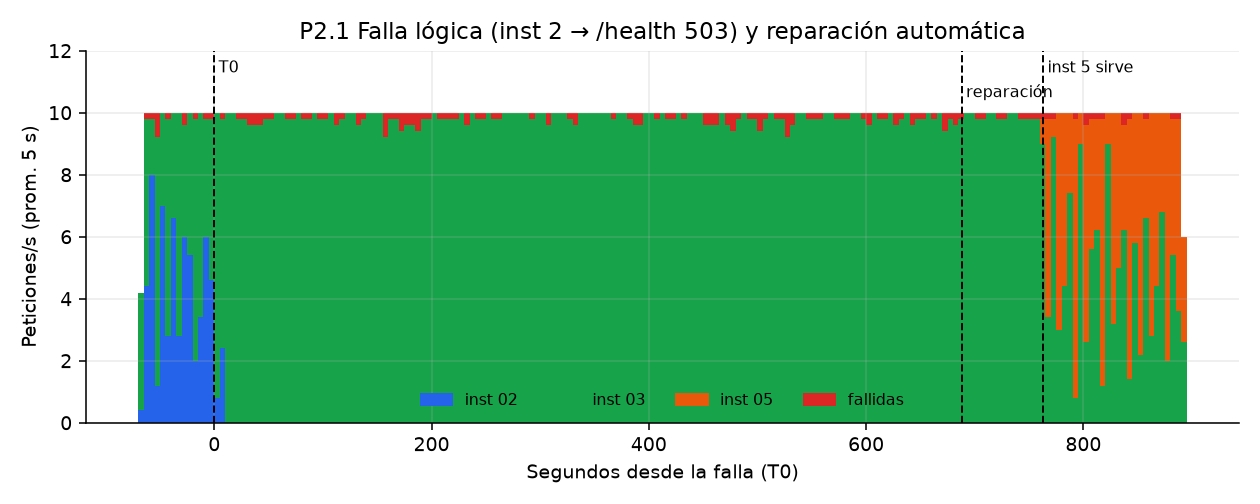
\includegraphics[width=\linewidth]{figuras/p2_logica.png}
\caption{Falla lógica.}
\end{subfigure}\hfill
\begin{subfigure}{0.49\textwidth}
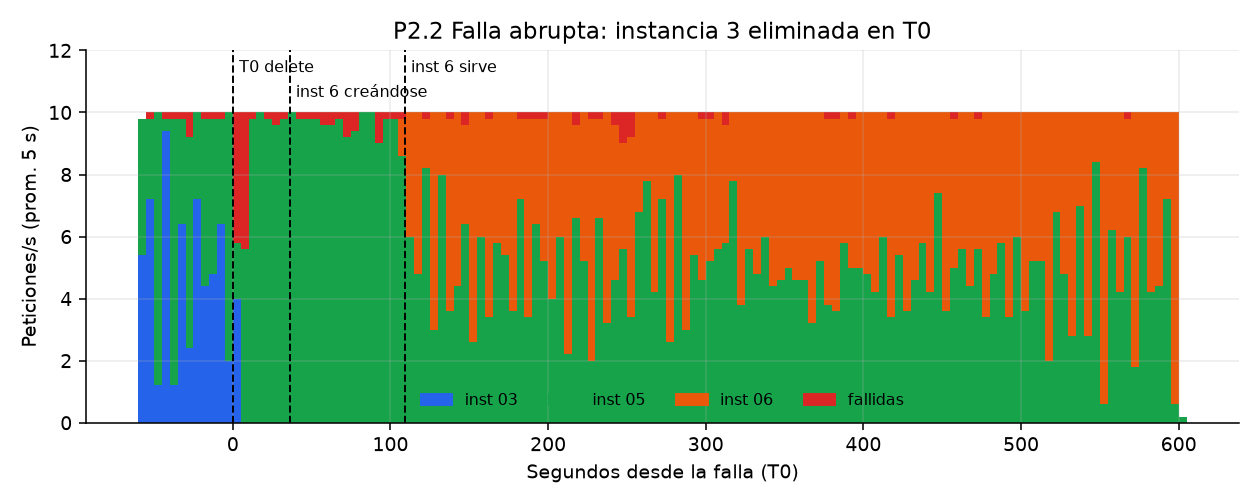
\includegraphics[width=\linewidth]{figuras/p2_abrupta.png}
\caption{Falla abrupta.}
\end{subfigure}
\caption{Peticiones por segundo que atendió cada servidor (colores) y las fallidas (rojo).}
\label{fig:p2}
\end{figure}

\begin{figure}[H]
\centering
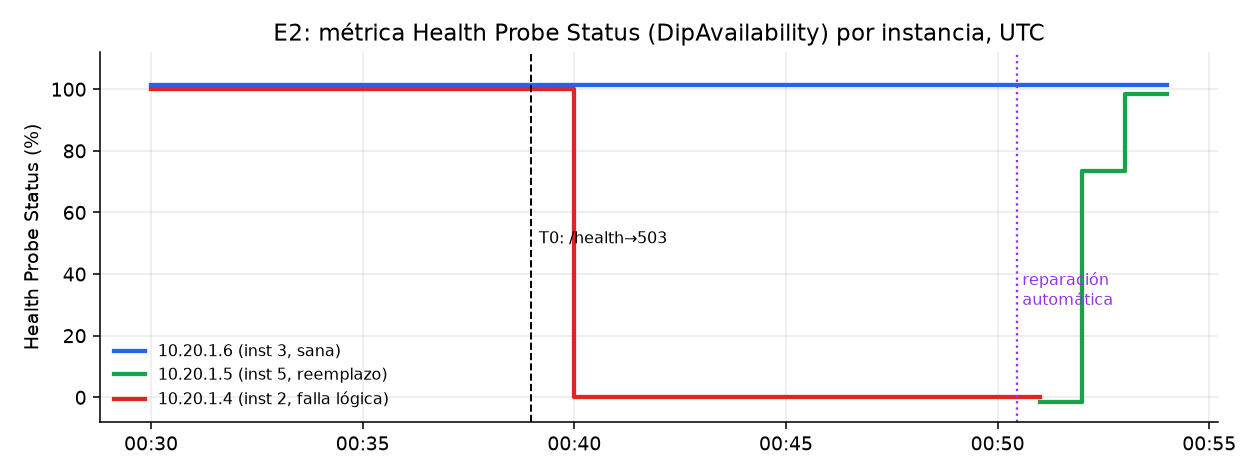
\includegraphics[width=0.6\textwidth]{figuras/e2_health_probe.png}
\caption{Salud de cada servidor según el balanceador: el servidor con falla queda en 0\,\% hasta que lo reemplazan.}
\label{fig:p2logica}
\end{figure}

\textbf{Análisis.} La falla lógica pasó desapercibida para los usuarios: el servidor siguió
respondiendo lo que tenía en curso mientras el balanceador lo retiraba, y el porcentaje de error
no cambió (esos pocos errores vienen de nuestra red doméstica y ya estaban antes de la falla). La
falla abrupta sí se notó, pero solo unos 15 segundos: es lo que tarda el balanceador en confirmar,
con dos revisiones de 5\,s, que el servidor ya no existe. Con más servidores en línea, la parte
afectada del tráfico sería menor. La reparación automática fue lenta (11 minutos) porque Azure
espera 10 minutos antes de reemplazar; el autoscale, en cambio, repuso la capacidad en menos de
2 minutos.


\subsection{P3 ¿Resisten los controles de seguridad?}
\begin{enumerate}
  \item \textbf{Leer el secreto desde otra red.} Desde Azure Cloud Shell, con un usuario que
        \emph{sí} tiene permiso sobre el Key Vault, la lectura fue rechazada por el firewall
        (\texttt{ForbiddenByFirewall}). Tener el permiso no basta: también hay que estar en una
        red autorizada.
  \item \textbf{Salir a Internet desde un servidor.} Desde dentro de una instancia, los intentos de
        conectar con \texttt{example.com} o \texttt{github.com} quedaron sin respuesta, mientras
        que el Key Vault sí respondió. El puerto SSH existe dentro de la máquina, pero no se puede
        alcanzar desde fuera.
  \item \textbf{Romper la política.} Intentamos crear una tarjeta de red con IP pública y un recurso
        en otra región; Azure rechazó ambos (Listado~\ref{lst:policy}).
\end{enumerate}

\begin{lstlisting}[caption={P3.3: Azure Policy rechaza los recursos prohibidos (salida abreviada).},label={lst:policy},language={}]
$ az network nic create ... --public-ip-address pip-prueba-violacion
ERROR: (RequestDisallowedByPolicy) ... "CaribeShop - Denegar NICs con IP publica"
$ az network nsg create ... -l westus
ERROR: (RequestDisallowedByPolicy) ... "CaribeShop - Solo region eastus"
\end{lstlisting}

\subsection{DevSecOps: un cambio inseguro bloqueado}
Cada cambio al código pasa por GitHub Actions, que revisa formato, validez y seguridad (Checkov).
Para comprobarlo abrimos a propósito un pull request que dejaba SSH abierto a Internet: Checkov lo
detectó (\texttt{CKV\_AZURE\_10}), el pipeline falló y el cambio no entró. Un segundo pull request
lo corrigió, usando el acceso de soporte de Azure en lugar de SSH, y se aprobó en verde.

\subsection{Auditoría (S6) y alertas (E5)}
\begin{lstlisting}[caption={S6: consulta KQL de lecturas del secreto y resultado.},label={lst:kql},language={}]
AzureDiagnostics
| where ResourceProvider == 'MICROSOFT.KEYVAULT' and OperationName == 'SecretGet'
| summarize Lecturas=count() by Identidad, Tipo=identity_claim_idtyp_s, Resultado=ResultSignature
-----------------------------------------------------------------------------------
Identidad             Tipo   Lecturas   Resultado
MI vmss-caribeshop    app    5          OK
operador (usuario)    user   1          OK
\end{lstlisting}

La consulta confirma que quien lee el secreto es la identidad de los servidores, desde la red
autorizada. Las alertas se dispararon cuando correspondía y llegaron por correo (Tabla~\ref{tab:alertas}).

\begin{table}[H]
\centering\small\tablaestilo
\caption{Alertas disparadas durante las pruebas.}
\label{tab:alertas}
\begin{tabular}{|l|c|c|c|}
\hline
\encab \hd{Alerta} & \hd{Gravedad} & \hd{Se activó (UTC)} & \hd{Se resolvió (UTC)} \\ \hline
Sonda de salud por debajo de 100\,\% & 2 & 23:14 & 23:30 \\ \hline
CPU alta sostenida & 3 & 23:53 & 00:00 \\ \hline
Sonda de salud por debajo de 100\,\% & 2 & 23:57 & 00:05 \\ \hline
Sonda de salud por debajo de 100\,\% & 2 & 00:12 & 00:26 \\ \hline
Sonda de salud por debajo de 100\,\% (P2.1) & 2 & 00:42 & 01:06 \\ \hline
\end{tabular}
\end{table}

% =================================================================
\section{SLA compuesto estimado}
% =================================================================
Para que una visita funcione deben estar disponibles, al mismo tiempo, la IP pública, el
balanceador y los servidores. Por eso la disponibilidad total se calcula multiplicando la de cada
uno (los servicios de monitoreo no influyen, porque no están en el camino de la visita).

\begin{table}[H]
\centering\small\tablaestilo
\caption{Disponibilidad garantizada por Microsoft para cada componente.}
\begin{tabular}{|l|c|}
\hline
\encab \hd{Componente} & \hd{SLA} \\ \hline
IP pública Standard & 99,99\,\% \\ \hline
Balanceador de carga Standard & 99,99\,\% \\ \hline
Servidores repartidos en 2 o más zonas & 99,99\,\% \\ \hline
Key Vault (solo para consultar la contraseña) & 99,99\,\% \\ \hline
\end{tabular}
\end{table}

\[
SLA_{\text{tienda}} = 0{,}9999^{3} = \mathbf{99{,}97\,\text{\%}}\quad(\approx 13\ \text{min de caída al mes})
\qquad
SLA_{\text{con Key Vault}} = 0{,}9999^{4} = 99{,}96\,\text{\%}
\]

Como comparación, con una sola máquina sin zonas (la situación del año pasado) el SLA sería de
99,5 a 99,9\,\%, es decir, entre 43 y 216 minutos de caída al mes solo por el servidor.

% =================================================================
\section{Riesgos aceptados}
% =================================================================
Checkov marca algunas configuraciones como mejorables. Las que decidimos no cambiar están
justificadas en el código con un comentario \texttt{\#checkov:skip}; la Tabla~\ref{tab:riesgos}
las agrupa por recurso.

\begin{table}[H]
\centering\footnotesize\tablaestilo
\caption{Riesgos aceptados, su justificación y cómo se mitigan.}
\label{tab:riesgos}
\begin{tabularx}{\textwidth}{|p{2.45cm}|Y|Y|c|}
\hline
\encab \hd{Regla} & \hd{Qué se aceptó y por qué} & \hd{Cómo se mitiga} & \hd{Riesgo} \\ \hline
\grupo{4}{Servidores y red} \\ \hline
\texttt{CKV\_AZURE\_97} & Sin cifrado extra en el host: requiere activar una función especial en la suscripción & Los discos ya están cifrados & Bajo \\ \hline
\texttt{CKV\_AZURE\_178} & Falso positivo: se usa llave SSH, no contraseña & El puerto 22 no es alcanzable & Nulo \\ \hline
\texttt{CKV\_AZURE\_160} & El puerto 80 abierto es la propia tienda; el tráfico no va cifrado & En producción: TLS y WAF & Medio \\ \hline
\grupo{4}{Key Vault} \\ \hline
\texttt{CKV2\_AZURE\_32} & Sin conexión privada (\emph{private endpoint}) & Firewall: solo la subred y el operador & Bajo \\ \hline
\texttt{CKV\_AZURE\_189} & Acceso público habilitado, pero filtrado por firewall & Probado en P3.1: otra red es rechazada & Bajo \\ \hline
\grupo{4}{Almacenamiento (app y estado de Terraform)} \\ \hline
\texttt{CKV\_AZURE\_206} & Réplica local, no en otra zona o región & Versionado y papelera de 7 días & Bajo \\ \hline
\texttt{CKV2\_AZURE\_1} & Cifrado con llaves de Microsoft, no propias & Cifrado AES-256 activo & Bajo \\ \hline
\texttt{CKV2\_AZURE\_33} & Sin conexión privada & Firewall y sin llaves compartidas & Bajo \\ \hline
\texttt{CKV\_AZURE\_59} & Acceso público habilitado, filtrado por firewall & Solo la subred y el operador & Bajo \\ \hline
\texttt{CKV\_AZURE\_33} & Registro de colas: no se usan colas & No aplica & Nulo \\ \hline
\texttt{CKV2\_AZURE\_21} & Registro de lecturas de blobs no necesario & Activarlo si se guardan datos de negocio & Bajo \\ \hline
\end{tabularx}
\end{table}

% =================================================================
\section{Costo mensual estimado en producción}
% =================================================================
Calculado con los precios públicos de Azure en East US (pago por uso, 730 horas al mes):

\begin{table}[H]
\centering\small\tablaestilo
\caption{Costo mensual estimado (USD).}
\label{tab:costo}
\begin{tabular}{|l|r|r|}
\hline
\encab \hd{Concepto} & \hd{Precio} & \hd{USD/mes} \\ \hline
\grupo{3}{Por cada servidor} \\ \hline
Máquina virtual D2s\_v4 (Linux) & 0,096 por hora & 70,08 \\ \hline
Disco del sistema & 2,40 al mes & 2,40 \\ \hline
\grupo{3}{Costos fijos} \\ \hline
Balanceador de carga & 0,025 por hora & 18,25 \\ \hline
IP pública & 0,005 por hora & 3,65 \\ \hline
Registros (Log Analytics, $\approx$\,2 GB) & 2,30 por GB & 4,60 \\ \hline
Key Vault, alertas y almacenamiento & -- & $<$\,2,50 \\ \hline
\grupo{3}{Total} \\ \hline
\textbf{Con 2 servidores} (mínimo) & & \textbf{$\approx$\,174} \\ \hline
\textbf{Con 4 servidores siempre encendidos} & & \textbf{$\approx$\,319} \\ \hline
\textbf{Con autoscale durante la campaña} & & \textbf{$\approx$\,202} \\ \hline
\end{tabular}
\end{table}

\textbf{Cómo ahorra el autoscale.} Si en la campaña se necesitan 4 servidores 4 horas al día,
3 servidores otras 4 horas y 2 el resto del día, se pagan unas 1\,800 horas de servidor al mes:
cerca de \textbf{USD 202}. Es \textbf{un 37\,\% menos} que dejar 4 servidores encendidos todo el
tiempo (USD 319), sin perder capacidad cuando hace falta.

% =================================================================
\section{Preguntas de análisis}
% =================================================================
\paragraph{1. ¿Cuántos servidores para 300 peticiones/s con respuestas en menos de medio segundo?}
Un servidor atiende 112 peticiones/s en menos de medio segundo, pero en ese punto su CPU está
casi al 100\,\%. Para tener margen conviene trabajar al 70\,\% (unas 62 peticiones/s por
servidor), lo que da $\lceil 300/62\rceil = $ \textbf{5 servidores}. Eso consume exactamente los
10 núcleos de nuestra cuota, así que \textbf{es viable, pero sin margen}. Para soportar además la
caída de una zona harían falta 6 (dos por zona). Lo que cambiaríamos: pedir más cuota a Azure
(al menos 16 núcleos), subir el máximo del autoscale a 6--8 y hacer la aplicación más eficiente
(caché de páginas, CDN para imágenes y un servidor web más rápido).

\paragraph{2. ¿Cuánto tardó el autoscale y qué hacer ante un pico a las 8:00 p.\,m.?}
Desde que la CPU superó el 70\,\% pasaron \textbf{5 min 19 s hasta que se ordenó el nuevo servidor}
y unos 6 minutos hasta que atendió tráfico. Ese tiempo es la suma de la ventana de 5 minutos que
usa para decidir, la demora de la métrica, la creación de la máquina y su instalación. Ante un pico
repentino serían varios minutos de lentitud. Proponemos:
\begin{itemize}
  \item \textbf{Perfil programado:} de 7:30 a 10:30 p.\,m. mantener al menos 4 servidores, para que
        la capacidad ya esté lista cuando empiece la campaña.
  \item \textbf{Autoscale predictivo:} Azure aprende de los últimos 7 días y agrega servidores antes
        del pico. Primero lo usaríamos solo en modo pronóstico para validarlo.
  \item \textbf{Reglas más rápidas} solo en ese horario: decidir con 2 minutos de datos, umbral del
        60\,\% y agregar 2 servidores a la vez.
\end{itemize}

\paragraph{3. ¿Cuál es ahora el punto único de falla?}
Dentro de la región no hay uno: la IP, el balanceador y los servidores están repartidos en tres
zonas. El punto único de falla es \textbf{la propia región East US}, porque todo vive en ella, y en
menor medida \textbf{el Key Vault}, que es uno solo (la aplicación guarda la contraseña 60\,s en
memoria, lo que solo cubre fallas cortas). Eliminarlo implica una copia de la plataforma en otra
región con Azure Front Door delante: unos USD 35/mes de Front Door más la segunda plataforma
(USD 100 a 174/mes). En total, entre 135 y 210 dólares más al mes, casi duplicar el costo.

\paragraph{4. Si un atacante lograra ejecutar código en un servidor, ¿qué podría hacer?}
\textbf{Podría} leer la contraseña de la base de datos (es la única que ese servidor puede leer),
alterar las respuestas de ese servidor o consumir su CPU. \textbf{No podría}:
\begin{itemize}
  \item leer otros secretos: el permiso está limitado a un solo secreto;
  \item cambiar la infraestructura: el servidor no tiene permisos de administración en Azure;
  \item entrar a otros servidores por SSH: no hay IPs públicas y la red solo deja pasar la web;
  \item enviar datos a un servidor propio en Internet: la salida está bloqueada (prueba P3.2);
  \item usar el almacenamiento: no tiene permisos y las llaves de acceso están desactivadas.
\end{itemize}
\textbf{Riesgo que queda:} la salida permitida hacia Storage abarca cualquier cuenta de la región,
incluso una del atacante. Se cerraría con conexiones privadas o un firewall que filtre por dominio.
Además, cada lectura del secreto queda registrada (S6), y tras un incidente se puede cambiar la
contraseña con un solo comando de Terraform.

\paragraph{5. ¿Por qué Checkov en el pipeline no reemplaza a Azure Policy, ni al revés?}
Porque protegen momentos distintos. \textbf{Checkov} revisa el código \emph{antes} de desplegar y
avisa temprano, pero solo ve lo que pasa por el repositorio: un cambio hecho a mano en el portal no
lo atraviesa, y un \texttt{\#checkov:skip} puede silenciarlo. \textbf{Azure Policy} actúa
\emph{dentro de Azure} y bloquea a cualquiera, venga de Terraform, del portal o de un atacante, pero
solo avisa en el momento de crear el recurso. Juntas cubren ambos frentes: en P3.3 la política
rechazó recursos creados por fuera de Terraform.

\paragraph{6. El estado de Terraform contiene secretos: ¿cómo se protegió?}
El archivo de estado guarda la contraseña generada, la llave SSH y el mapa de la infraestructura.
Lo protegimos así:
\begin{itemize}
  \item vive en Azure, nunca en el computador ni en Git;
  \item la cuenta no acepta llaves de acceso: solo entra quien tenga identidad y permiso en Azure;
  \item firewall limitado a nuestras IPs, cifrado y conexión segura;
  \item historial de versiones y papelera de 7 días, y bloqueo para que dos personas no lo editen
        a la vez.
\end{itemize}
Si se filtrara, el atacante tendría la contraseña y la llave SSH (inútil, porque el puerto 22 no es
alcanzable) y conocería la arquitectura. Habría que cambiar la contraseña, regenerar la llave y
revisar los registros de acceso. Como mejora, las versiones recientes de Terraform permiten que
los secretos nunca se guarden en el estado.

% =================================================================
\section{Conclusiones}
% =================================================================
La plataforma resuelve los tres problemas de CaribeShop, y cada solución se comprobó con datos.
Ante la \textbf{saturación}, el autoscale pasó de 2 a 4 servidores y volvió a 2 con solo 0,55\,\%
de errores. Ante la \textbf{falla de una máquina}, un servidor enfermo salió de circulación en
8 segundos sin que los usuarios lo notaran, y cuando borramos uno de golpe la capacidad se
recuperó en menos de 2 minutos. Ante la \textbf{auditoría}, ya no hay secretos en el código ni
accesos de administración expuestos, y el pipeline bloqueó un cambio que intentaba abrir SSH.

La seguridad se construyó en capas, y cada una se puso a prueba intentando romperla. Medir cuánto
aguanta un servidor nos permitió justificar la configuración del autoscale y responder cuántos se
necesitan para 300 peticiones por segundo. La principal limitación es que el autoscale tarda unos
5 a 6 minutos en reaccionar, algo que en una campaña se resuelve programándolo con anticipación.
Al terminar eliminamos todos los recursos con \texttt{terraform destroy}. Las capturas y salidas
de comandos que respaldan cada requisito están en la carpeta \texttt{evidencias/} del repositorio.


\end{document}
